%%%%%%%%%%%%%%%%%%%%%%%%%%%%%%%%%%%%%%%%%%%%%%%%%%
%
% LaTeX Template for extended abstracts for the
% ISSW 2023 in Bend, Oregon.  
%   Slight modifications to the amazing template by the 2018 ISSW organizers, in particular JT Fischer.  THANK YOU!
%
%%%%%%%%%%%%%%%%%%%%%%%%%%%%%%%%%%%%%%%%%%%%%%%%%%
%               * INSTRUCTIONS *
%
%           **** VERY IMPORTANT ****
%
%
%  1 - Rename this file
%  
%  2 - Write your contribution
%
%  3 - Compile it with pdflatex or latex
%
%  4 - Follow instructions below and come to Innsbruck
%%%%%%%%%%%%%%%%%%%%%%%%%%%%%%%%%%%%%%%%%%%%%%%%%%

\documentclass[3p,authoryear,times,twocolumn]{elsarticle_issw2018}

% include packages as needed, such as
\usepackage[utf8]{inputenc}
\usepackage{amsmath,amssymb,amsfonts}
\usepackage{graphicx,color}

\begin{document}

\begin{frontmatter}

\title{INSTRUCTIONS FOR FORMATTING YOUR EXTENDED ABSTRACT\\INTERNATIONAL SNOW SCIENCE WORKSHOP 2023, BEND, OREGON, USA}

\author[1]{Depthina A. Hoar\corref{complete_address}}
\cortext[complete_address]{Corresponding author address:\\Depthina A. Hoar, Institute of Hoarticulture,\\Walla Walla, WA 98523-1234;\\tel: +1 509-555-1234; fax: +1 509-555-1235\\
email: dhoar@depth.snow}
\author[2]{Precipina B. Particle}
\author[3]{Surfer C. Hoar}

\address[1]{Institute of Hoarticulture, Walla Walla, WA, USA}
\address[2]{Avalanche Forecasting Centre, Skookumchuk, BC, Canada}
\address[3]{Highway Safety Office, Brunico, Italy}

\begin{abstract}
\noindent
These instructions are laid-out in the same format as is requested for ISSW 2023 conference proceedings. The abstract should be less than 250 words. It can be either the same as your initial short abstracts or you can make changes as you wish, for example include new results you have obtained since your initial submission.
\end{abstract}

\begin{keyword}
Select 3-6 keywords.
\end{keyword}

\end{frontmatter}

% ===================================================================================================
\section{INTRODUCTION}
All ISSW presenters - both oral and poster presenters - are required to submit a paper (maximum 8 pages) that describes their presentation topic in more detail for publication in the ISSW 2023 proceedings. At this ISSW, the conference proceedings will only be published electronically.
%
% ===================================================================================================
\section{MANUSCRIPT DEADLINE}
Manuscripts must be received by \textbf{\underline{August 31, 2023}.}\\

\noindent
We cannot guarantee that late papers will be included in the conference line-up and the proceedings publication. \textbf{Your oral or poster presentation slot is conditional on us receiving your paper by this date.}
%
% ===================================================================================================
\section{LANGUAGE} 
Authors are greatly encouraged to submit their papers in English, since they have a far wider reach.
%
% ===================================================================================================
\section{PAGE LIMIT, LAYOUT \& TEXT FONT}
Papers are limited to \textbf{\underline{no more than 8 pages}}, including references, appendices, etc.  must be formatted on A4 pages (210 mm x 297 mm) with 2.5 cm (about 1 inch) margins on all sides. In word, please use the styles and formatting templates provided within this document (‘ISSW - …’), or 10-point Arial for the text body.
Place the text in newspaper style columns with a 0.8 cm space between columns. If necessary, figures, photos, or charts may span the two columns, adhering to the 2.5 cm margins.

%
\subsection{Titles, headings and footnotes}
The title of the paper should be centered and typed in CAPITAL LETTERS on the first line of your first page of your manuscript. Type the name of all the author(s) in initial caps and center on the page two lines below the title. Type the author's affiliation, city, and country on the line below their name in initial caps.\\
%

\noindent
Major headings are Arabic-numbered in CAPITAL LETTERS (as shown in these instructions). Secondary headings are in italics and underlined (as shown in these instructions). Footnotes should be indicated in the text with an asterisk (*).\\
%
\noindent
Do not include any page numbers, headers or footers in your manuscript.
%
\subsection{Author's corresponding address}
Please type, within the 2.5 cm margin, the corresponding author's address in the lower left corner of your first page (see lower left corner of the first page of these instructions).
%
\subsection{References}
List all bibliographic references at the end of the paper in alphabetical order by first author. When referring to them in the text, type the corresponding author's surname, followed by the year of publication, e.g. \cite{McClung2006}. When there are three or more authors, use the first author's name followed by "et al.", e.g. \cite{Greene2006} as an example of a proceedings paper or \cite{Fischer2022} as an example of a journal paper. Use referencing style as used in Natural Hazards and Earth System Sciences (see sample references at the end of these instructions).

%
\subsection{Equation numbers}
Enclose these Arabic (and sequential) numbers in parentheses and place flush with right-hand margin of column.
%
\subsection{Units}
The International System of Units (SI units) should be used in the ISSW Proceedings.
%
% ===================================================================================================
\section{FIGURES, TABLES AND CAPTIONS}
Presentations at the conference do not usually allow enough time for in-depth understanding; therefore, it is important to include your most complex graphs, diagrams, etc., in your extended abstract.\\
%

\noindent
Figures and tables should be reduced so that they may be incorporated into the text along with the appropriate pages, with full captions typed in (see Figure \ref{fig.issw_logo}).\\

\noindent
All color photographs should be in RGB color space, and at least 160 ppi at the size shown in your manuscript. A table or figure that cannot be placed in the same orientation as the text should be rotated 90 degrees counter-clockwise so that the figure and caption may be read by rotating the published proceedings 90 degrees clockwise. \\

\noindent
Company logos and identification numbers are not permitted on your illustrations.
\begin{figure}[ht]
 \centering
 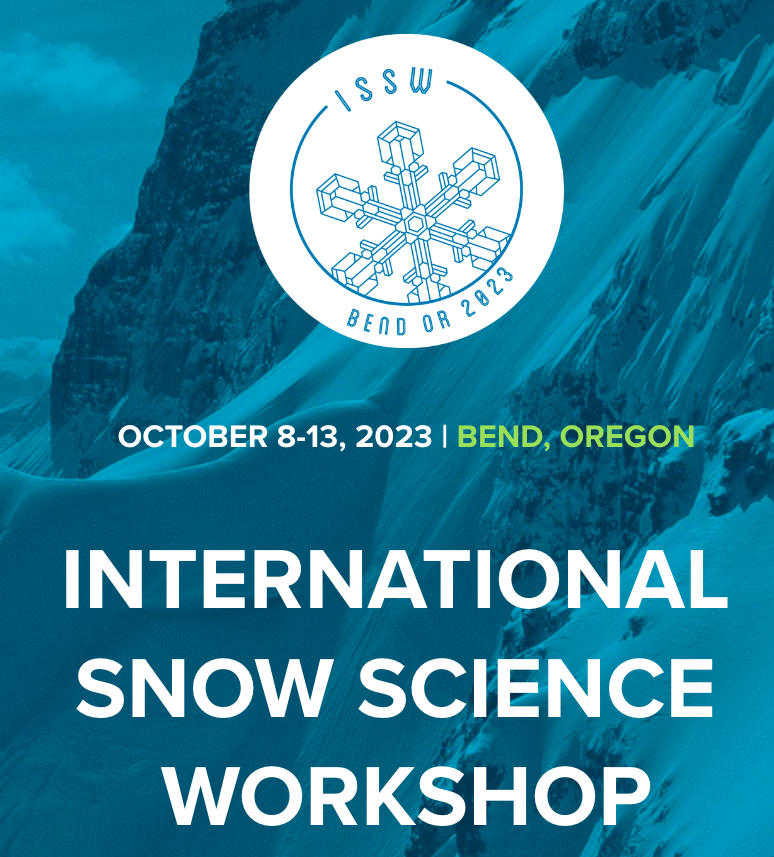
\includegraphics[width=0.75\columnwidth]{./issw_logo}
 \caption{The International Snow Science Workshop (ISSW) 2023 is taking place in Bend, Oregon.}
 \label{fig.issw_logo}
\end{figure}
% ===================================================================================================
\section{SUBMISSION}
If you created your manuscript in Word or other word processing software such as LaTex, \textbf{\underline{convert your manuscript to}} \textbf{\underline{PDF file format}}. No other formats are accepted.\\

%
\noindent
Check the manuscript to ensure nothing changed during the conversion process. Always review formatting, citations, figures, tables, and equations closely in the PDF after converting.\\

%
% ===================================================================================================
\section{QUESTIONS}
For questions about the submission process, please contact Nadia Leamy (nadia@icsevents.com). \\
%
\noindent
%
For questions about formatting and content, please contact Erich Peitzsch (erich@issw2023.com) or HP Marshall (hpmarshall@boisestate.edu). % ===================================================================================================
\section*{ACKNOWLEDGEMENT} 
Thank You.
% ===================================================================================================

\bibliographystyle{Copernicus}  % style file from NHESS
\bibliography{issw_bibliography}



%%%%. IF YOU WANT TO DO BIBLIOGRAPHY BY HAND, UNCOMMENT BELOW
%\section*{REFERENCES}
%\bibliographystyle{apalike}
%\renewcommand{\section}[2]{} % delete bibliography title
%\begin{thebibliography}{}
%
%\bibitem[Greene et al. (2006)]{Greene2006}
%Greene, E., T. Wiesinger, K. W. Birkeland, C. Coleou, A. Jones, and G. Statham.
%\newblock {Fatal avalanche accidents and forecasted danger levels: Patterns in the United States, Canada, Switzerland and France.}
%\newblock {\em Proceedings of the International Snow Science Workshop, Telluride, CO}, , 640-649, 2006.
%
%\bibitem[McClung and Schaerer, 2006]{McClung2006}
%McClung, D.~M. and Schaerer, P.
%\newblock {\em {The avalanche handbook}}.
%\newblock The Mountaineers Books, Seattle, WA, 3rd edition edition, 2006.
%
%\bibitem[Fischer et al. (2022)]{Fischer2022}
%Fischer, K. C., Haegeli, P., and Mair, P.
%\newblock {Travel and terrain advice statements in public avalanche bulletins: a quantitative analysis of who uses this information, what makes it useful, and how it can be improved for users.}
%\newblock {Nat. Hazards Earth Syst. Sci, 22, 1973-2000, https://doi.org/10.5194/nhess-22-1973-2022, 2022}
%
%\end{thebibliography}


% ===================================================================================================
\end{document}
% --- THIS IS THE END MY FRIEND ---
% ===================================================================================================

